%!TEX program = xelatex
% 完整编译: xelatex -> biber/bibtex -> xelatex -> xelatex
\documentclass[lang=cn,a4paper]{elegantpaper}
\ExecuteBibliographyOptions{sorting=none}
\title{人工智能编程5}
\author{彭程~~ 2020011075 \\ 清华大学~~ 自动化系~~ 自02班}
%\institute{\href{https://elegantlatex.org/}{Elegant\LaTeX{} 项目组}}

%\version{0.10}
\date{\zhtoday}

\usepackage{float}
% 本文档命令
\usepackage{array}
\newcommand{\ccr}[1]{\makecell{{\color{#1}\rule{1cm}{1cm}}}}
\addbibresource[location=local]{reference.bib} % 参考文献,不要删除
\usepackage{outlines}
\usepackage{color}



\begin{document}

\maketitle

\begin{abstract}
本文为2022秋《人工智能基础》编程5的实验报告。本次作业使用强化学习方法完成游戏迷宫求解。
\keywords{RL,Q-Learning,Sarsa}
\end{abstract}

\section{问题建模}

\subsection{状态空间}
利用老鼠所在的格子定义状态,所给问题中共有 25 个格子,故状态空间:
$$S = \{ (x, y)|0 \le x \le 4, 0 \le y \le 4 \}$$
\subsection{行动集合}
根据题意,行动集合为$ A = \{up, down, left, right\}$
\subsection{状态转移概率}
当老鼠在状态 $s_t$ 采取动作 $a$ 时,将根据动作对应的方向 (向上、向下、向左、向右),以概率 1 转移
到 $s_{t+1}$ 中,需要注意的是,如果动作 a 会使老鼠移出环境方格,则老鼠的状态保持不变。
若向上、向下、向左、向右的概率分别为 p1、 p2、 p3、 p4,则向对应状态转移的概率也对应为 p1、 p2、p3、 p4。$p_{ss'}^a = P(S_{t+1} = s' | S_t = s, A_t = a)$,当状态和行动指定时,状态转移概率是确定的。
\subsection{回报}
定义老鼠移动一步的回报 $R_t = -1$,老鼠到达陷阱的回报 $R_t = -5$,老鼠撞墙获得的回报$R_t = -2$,老鼠到达终点的回报 $R_t = 10$。


\section{编程求解}
\subsection{Q-Leaning}

Q-Leaning 方法的行动价值递推公式为:
$$
Q\left(S_{t}, A_{t}\right) \leftarrow Q\left(S_{t}, A_{t}\right)+\alpha\left(R_{t+1}+\gamma \max_a Q\left(S_{t+1}, a\right)-Q\left(S_{t}, A_{t}\right) \right)
$$

利用 $ \epsilon -greedy$算法选择行为策略,  公式为:
$$
\left\{\begin{array}{l}
\pi(a \mid s)=1-\epsilon+\frac{\epsilon}{m}, \quad \text { if } a=\operatorname{argmax}_{a \in A} Q(s, a) \\
\pi(a \mid s)=\frac{\epsilon}{m}, \quad \text { otherwise }
\end{array}\right.
$$


接下来编程实现$\epsilon - greedy$的Q-Leaning算法。定义折现因子 $\gamma = 0.5$,$\epsilon = 0.01$,$lr(\alpha) = 0.1$,运行100个episode的结果如下(纵列0123分别代表上下右左,横排坐标为状态(x,y)):


% Table generated by Excel2LaTeX from sheet 'Sheet1'
\begin{table}[htbp]
  \centering
  \caption{Q-Learning行动价值表}
    \begin{tabular}{ccccc}
      \hline
                  &         0&         1&         2&         3 \\
    \hline
    (0,0) & -1.837978& -1.733839& -1.752091& -1.838560 \\
     (0,1)& -1.601735& -1.574143& -1.571919& -1.585546 \\
     (0,2)& -1.346318& -1.355000& -1.143002& -1.252222 \\
     (0,3)& -0.741975&  0.040822& -0.752725& -0.754186 \\
     (0,4)& -0.570500& -0.567380& -0.570500& -0.638154 \\
     (1,3)& -0.301156&  3.046926& -0.285500& -0.500000 \\
     (1,0)& -1.564576& -1.418010& -1.559048& -1.603054 \\
     (2,0)& -1.162537& -0.703059& -1.355000& -1.206651 \\
     (2,2)&  0.000000&  0.000000&  0.000000&  0.000000 \\
     (1,1)& -1.543758& -1.719500& -1.719500& -1.553839 \\
    (1,4) & -0.393233& -0.348900& -0.390000& -0.356430 \\
     (2,4)& -0.199500& -0.190000& -0.200000& -0.095000 \\
     (3,0)& -0.598374& -0.640006&  0.819091& -0.741975 \\
     (4,0)& -0.469564& -0.570500& -0.498877& -0.570500 \\
     (4,1)& -0.318554& -0.390000& -0.280500& -0.290060 \\
     (3,1)& -0.500000& -0.199500&  3.894217& -0.109500 \\
     (3,2)&  9.969567& -0.100000&  0.000000&  0.000000 \\
     (4,2)&  0.044280& -0.200000& -0.100000& -0.195000 \\
     (4,3)& -0.100000&  0.000000& -0.100000& -0.100000 \\
     (3,3)& -0.100000& -0.100000&  0.000000& -0.050000 \\
     (2,3)& -0.105000& -0.100000& -0.100000&  9.528987 \\
     (3,4)& -0.105000& -0.100000& -0.200000& -0.100000 \\
     (4,4)& -0.100000& -0.200000& -0.200000& -0.100000 \\
    \hline
    \end{tabular}%
  \label{tab:addlabel}%
\end{table}%

\begin{figure}[H]
  \centering
  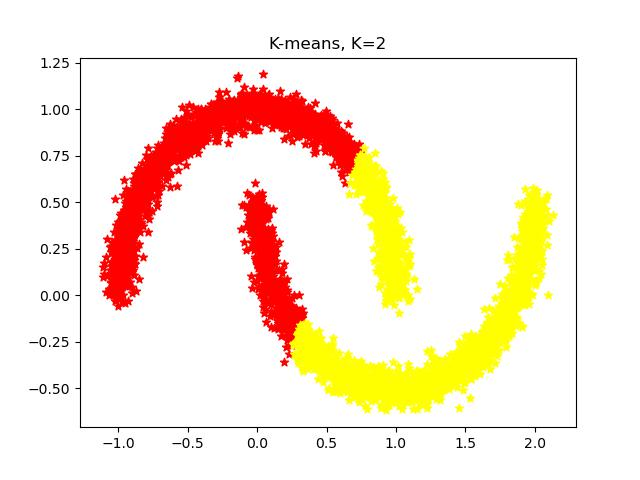
\includegraphics[width=0.5\textwidth]{1.jpg}
  \caption{Q-Learning最优行动序列} 
  \label{Fig.1}
\end{figure}




\subsection{Sarsa}

Sarsa 方法的行动价值递推公式为:
$$
Q\left(S_{t}, A_{t}\right) \leftarrow Q\left(S_{t}, A_{t}\right)+\alpha\left(R_{t+1}+\gamma Q\left(S', A'\right)-Q_{S_{t}, A_{t}}\right)
$$
利用  $\epsilon -greedy$算法选择行为策略,  公式为:
$$
\left\{\begin{array}{l}
\pi(a \mid s)=1-\epsilon+\frac{\epsilon}{m}, \quad \text { if } a=\operatorname{argmax}_{a \in A} Q(s, a) \\
\pi(a \mid s)=\frac{\epsilon}{m}, \quad \text { otherwise }
\end{array}\right.
$$

接下来编程实现$\epsilon - greedy$的Sarsa算法。定义折现因子 $\gamma = 0.5$,$\epsilon = 0.01$,$lr(\alpha) = 0.1$,运行100个episode的结果如下(纵列0123分别代表上下右左,横排坐标为状态(x,y)):

% Table generated by Excel2LaTeX from sheet 'Sheet1'
\begin{table}[htbp]
  \centering
  \caption{Sarsa行动价值表}
    \begin{tabular}{ccccc}
    \hline
                    &      0   &      1     &    2     &    3 \\
    \hline
    (0,0) & -1.837746& -1.751700& -1.759316& -1.838560 \\
     (0,1)& -1.599047& -1.562262& -1.546094& -1.585078 \\
     (0,2)& -1.206651& -1.355000& -1.013137& -1.205571 \\
     (1,0)& -1.594765& -1.466272& -1.556852& -1.605052 \\
     (1,1)& -1.539618& -1.719500& -1.719500& -1.529736 \\
     (2,0)& -1.215911& -0.789449& -1.355000& -1.206651 \\
     (3,0)& -0.772834& -0.697010&  0.702922& -0.741975 \\
     (3,1)& -0.500000& -0.100000&  3.800872& -0.109750 \\
     (4,1)& -0.260731& -0.390000& -0.280500& -0.304224 \\
     (4,2)& -0.100000& -0.200000& -0.190000& -0.200000 \\
    (3,2) &  9.929303& -0.100000& -0.091957&  0.000000 \\
     (4,3)& -0.190000& -0.200000& -0.100000& -0.100000 \\
     (2,2)&  0.000000&  0.000000&  0.000000&  0.000000 \\
     (0,3)& -0.741975&  0.344538& -0.701937& -0.681059 \\
     (0,4)& -0.570500& -0.498877& -0.570500& -0.556076 \\
     (1,4)& -0.290058& -0.357450& -0.390000& -0.281645 \\
     (1,3)& -0.208750&  3.453045& -0.195000& -0.500000 \\
     (2,3)& -0.100000&  0.000000& -0.100000&  9.797244 \\
     (2,4)& -0.199750& -0.190000& -0.200000& -0.140000 \\
     (3,4)& -0.100000&  0.000000& -0.200000& -0.100000 \\
     (4,0)& -0.568269& -0.570500& -0.498514& -0.570500 \\
     (3,3)&  0.530860& -0.100000&  0.000000& -0.050000 \\
     (4,4)&  0.000000&  0.000000&  0.000000& -0.105000 \\
     \hline
    \end{tabular}%
  \label{tab:addlabel}%
\end{table}%
\begin{figure}[H]
  \centering
  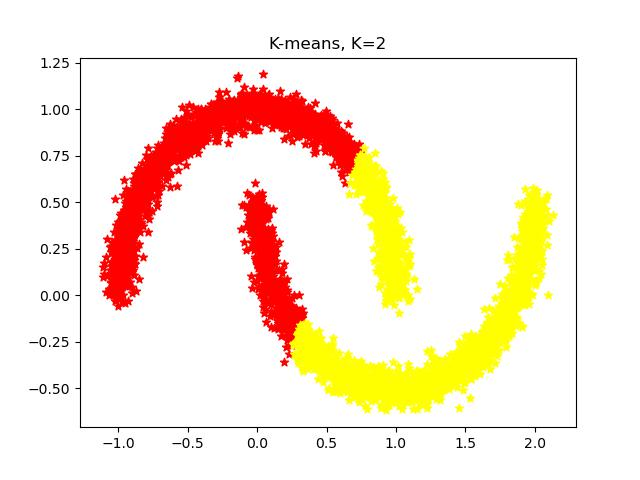
\includegraphics[width=0.5\textwidth]{1.jpg}
  \caption{Sarsa最优行动序列} 
  \label{Fig.1}
\end{figure}


\section{思考题}

\noindent \textbf{如果环境是动态的,例如老鼠夹的个数和位置会随时间变化,该如何求解这个问题?请简述你的想法,本问无需编程实现。}


\noindent 1. 可以考虑增大折现因子和学习率,使得后续训练过程中环境的更新对 Q 表的影响更大;

\noindent 2. 可以采用蒙特卡洛或者时序差分,从经验中去学习,做实验模拟得到样本的状态、动作和奖励序列,通过平均所有样本的回报得到行动价值,并更新策略。

\noindent 3.传统算法的状态空间的大小将急剧增大,可以考虑采用 DQN 等深度强化学习网络进行学习





% \begin{lstlisting}[title = 静态数据增强 ,language = python]
%   def image_pro(path):
%     image0 = Image.open(path)
% \end{lstlisting}




% \begin{figure}[H]
%   \centering
%   \includegraphics[width=0.9\textwidth]{data对比.png}
%   \caption{有无数据增强对比} 
%   \label{Fig.1}
% \end{figure}



\nocite{*}
\printbibliography[heading=bibintoc, title=\ebibname]

\appendix
%\appendixpage
\addappheadtotoc

\end{document}
